\documentclass{article}

% Language setting
% Replace `english' with e.g. `spanish' to change the document language
\usepackage[french]{babel}
\usepackage[fleqn]{amsmath} % Aligner les équations à gauche


% Set page size and margins
% Replace `letterpaper' with`a4paper' for UK/EU standard size
\usepackage[letterpaper,top=2cm,bottom=2cm,left=3cm,right=3cm,marginparwidth=1.75cm]{geometry}

% Useful packages

\usepackage{amsmath}
\usepackage{graphicx}
\usepackage{subcaption}
\usepackage[colorlinks=true, allcolors=blue]{hyperref}

\title{TD 1 - Optique géométrique }
\author{IPESUP - PC }
\date{DATE }

\begin{document}
\maketitle



\section{Rappels de cours}

\begin{itemize}
  \item Loi de Snell-Descartes pour la réflexion : lors d'un changement de milieu (d'indice $n_1$ à $n_2$), le rayon réfracté appartient au plan formé par le rayon incident et la normale au point d'incidence. Les angles $i$ et $r$ entre la \textbf{normale} et le \textbf{point d'incidence} respectent la relation suivante $\frac{\sin(i)}{\sin(r)} = \frac{n_2}{n_1}$
  \item Relation de conjugaison de Descartes: $\frac{1}{\overline{OA'} } - \frac{1}{\overline{OA} } = \frac{1}{f'}$. Attention aux signes ! 
  \item Relation de Newton : $\overline{F'A'} \times \overline{FA} = -f'^2$
\end{itemize}

\textbf{Anecdote: }À la fin du XVIII° siècle, les télescopes réfracteurs (utilisant des lentilles) présentaient un problème majeur appelé l'aberration chromatique, où les différentes couleurs de la lumière se focalisaient à des points différents, rendant les images floues. Isaac Newton, insatisfait de cette limitation, décida de concevoir un télescope utilisant des miroirs au lieu de lentilles. En 1668, il construisit le télescope réflecteur de Newton, qui utilisait un miroir concave pour réfléchir la lumière et une petite lentille plate pour diriger l'image vers l'oculaire.
Le télescope réflecteur de Newton est encore largement utilisé aujourd'hui et constitue une application emblématique de l'optique géométrique. 
\section{Chemins optiques}

La lentille (L) est en verre d'indice $n$ et de centre optique $O$.
Elle a une épaisseur $e$ au niveau du centre optique. 
Soit $f'$ la distance focale de la lentille et $n_{air}$ l'indice optique de l'air.
Soient $M$ et $M'$ deux point de l'espace dont les coordonnées sont respectivement $(x,0)$ et $(x',y')$.
On place une source de lumière $S$ devant la lentille sur l'axe $(Ox)$. 
\begin{enumerate}
  \item On suppose que $OS=f'$. Représenter le schéma de la situation et construire les rayons issus de $S$ qui parviennent en $M$ et $M'$. Exprimer $(SM)$ et $(SM')$ les chemins optiques. 
  \item Même question si $OS=\frac{3f'}{2}$.
\end{enumerate}




\begin{figure}[h]
  \centering
  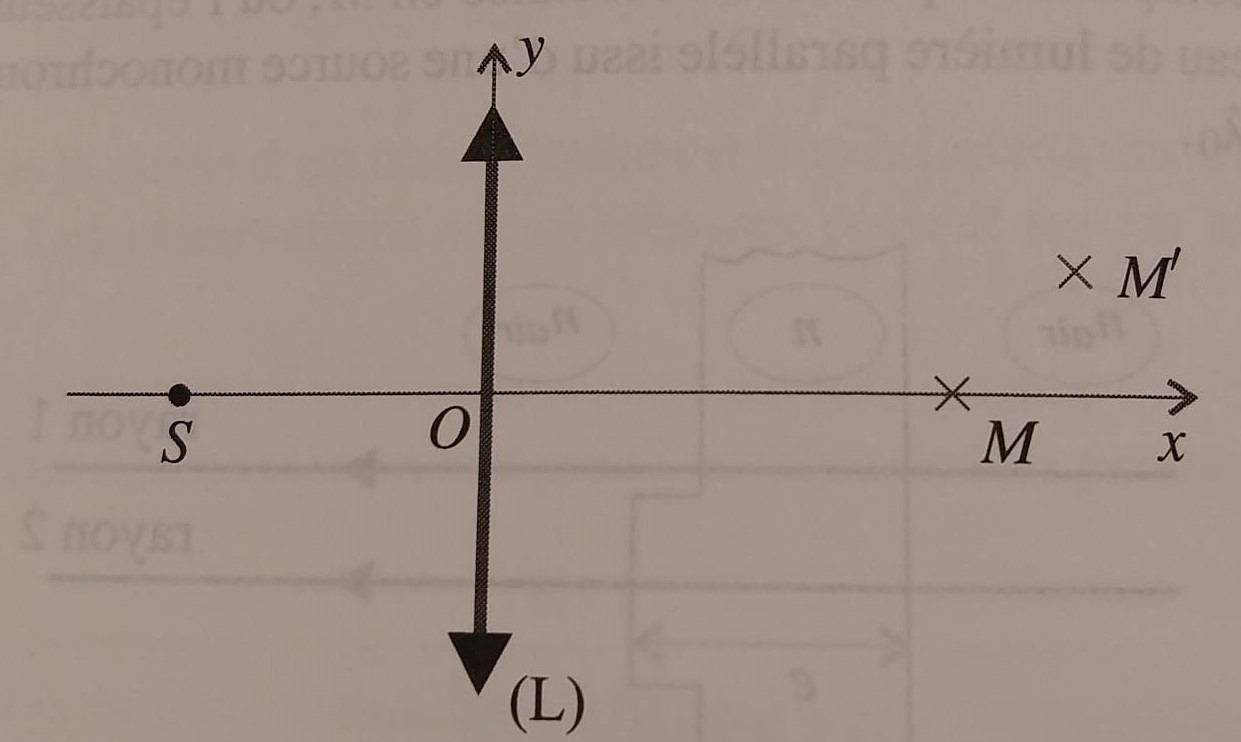
\includegraphics[width=0.3\textwidth]{exercice 1.jpg}
  \label{fig:ex}
    \caption{Schéma de la lentille}
\end{figure}


\section{Modèle d'une cavité}

On modélise une cavité optique par une suite de lentilles convergentes identiques de focale $f'$, coaxiales, et séparées d'une distance $a$. 
La lentille $n$ est frappée au point d'abscisse $y_n$ par un rayon lumineux.
L'angle entre l'horizontale et le rayon lumineux est noté $\alpha_n$ et est compté positivement dans le sens direct. 
\begin{enumerate}
  \item Déterminer deux relations de récurrence entre $y_{n+1}$ et $y_n$, $\alpha_{n+1}$ et $\alpha_n$ puis en déduire une relation d'ordre 2 sur les $y_n$. 
  \item A quelle condition sur $a$ et $f$ le dispositif est-il intéressant ? 
  \item Résoudre le problème dans le cas où $a=2f$.
\end{enumerate}

\begin{figure}[h!]
  \centering
  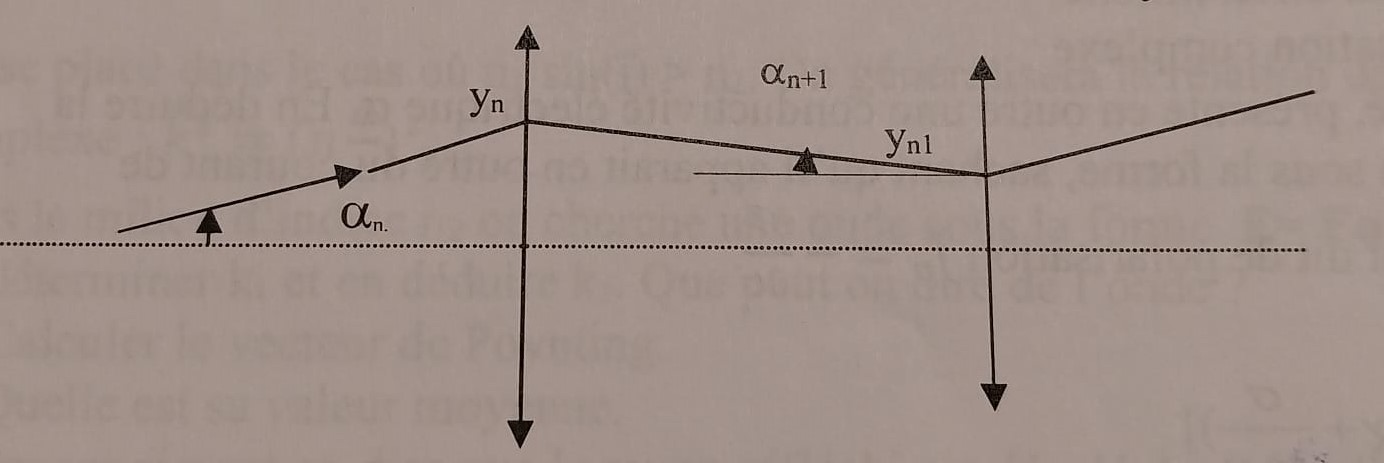
\includegraphics[width=0.4\textwidth]{exercice 2.jpg}
    \caption{Schéma de la cavité}
\end{figure}


\section{Fibre optique}

On considère une fibre optique orientée selon l'axe $(Oz)$ dont le milieu est d'indice variable $n(r)=n_0 \sqrt{1-(\frac{kr}{a})^2}$ et dont la gaine est d'indice $n_G$. 
\begin{enumerate}
  \item Déterminer $k$ pour avoir continuité de l'indice. 
  \item Pourquoi peut-on se placer dans le plan $(Ozx)$ ? 
  \item On considère un rayon incident sur une strate $r=cte$ d'angle d'incidence $i$. Montrer qu'on a alors $n(r)sin(i) = C$. 
  \item En déduire que $(\frac{dr}{dz})^2 = A n(r)^2 - 1$, avec $A$ une constante à déterminer. 
  \item Déterminer $r(z)$ l'équation de la trajectoire d'un rayon lumineux. 
\end{enumerate}


\begin{figure}[h!]
  \centering
  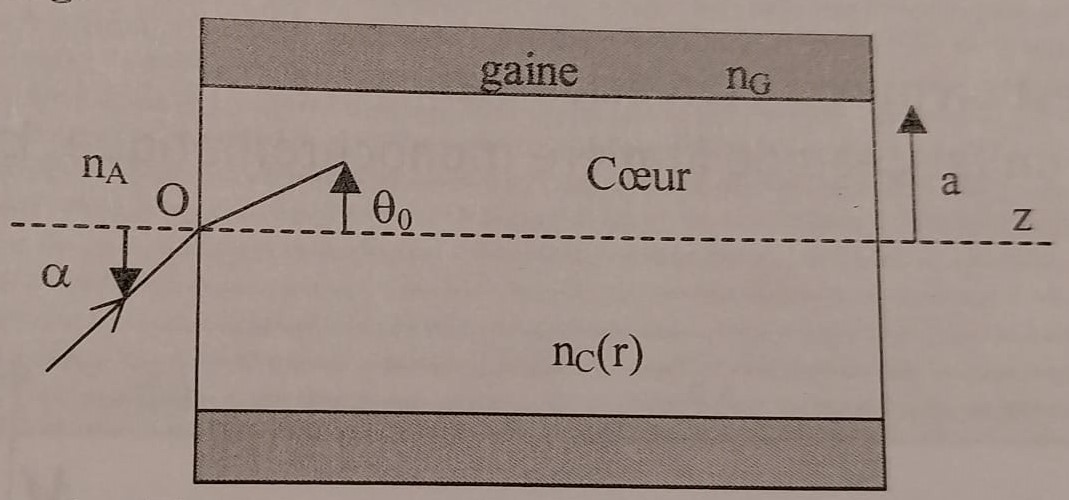
\includegraphics[width=0.4\textwidth]{exercice 3.jpg}
    \caption{Schéma de la gaine}
\end{figure}

\newpage
\section{Prisme}

On considère un prisme isocèle d'angle au sommet A et d'indice $n$ plongé dans l'air d'indice 1, traversé par un rayon lumineux. 
On note $i$ l'angle d'incidence, $r$ l'angle de réfraction sur la première face, $i'$ l'angle à la sortie du prisme et $r'$ l'angle d'incidence sur la deuxième face. On note $D$ l'angle de déviation total. 

\begin{figure}[h]
  \centering
  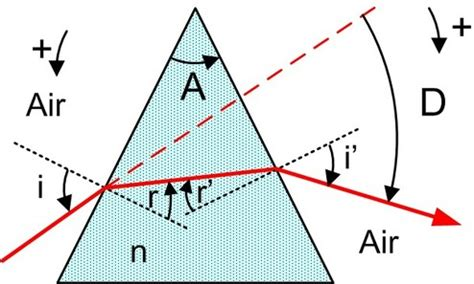
\includegraphics[width=0.45\textwidth]{prisme.jpeg}
  \caption{Schéma du prisme}
\end{figure}
\begin{enumerate}
  \item Faire un schéma de la situation et déterminer les relations entre $i$, $r$, $i'$ et $r'$.
  \item Déterminer une relation entre $A$, $r$ et $r'$ d'une part et $D$, $A$, $i$ et $i'$ d'autre part.
  \item Montrer que $D$ s'exprime en fonction de $i$ uniquement.
  \item Expérimentalement, on observe un unique minimum de déviation $D_{min}$ quand on fait varier l'angle d'incidence $i$, obtenu pour $i=i_{min}$. Par un argument de symétrie, en déduire qu'on a nécessairement $i=i'$ au minimum de déviation. 
  \item Exprimer $n$ en fonction de $A$ et $D_{min}$.\\[1cm]
\end{enumerate}

\begin{figure}[h]
  \centering
  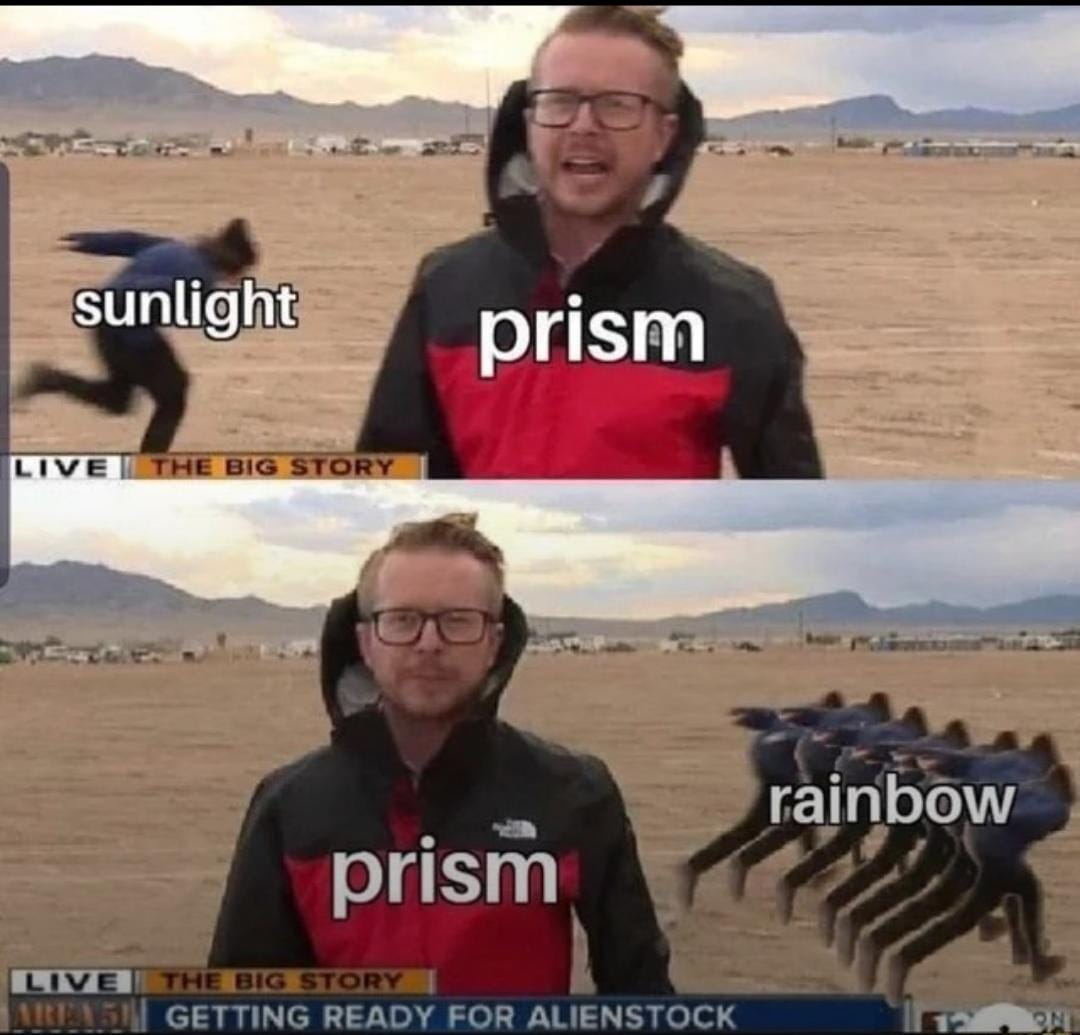
\includegraphics[width=0.55\textwidth]{prisme.jpg}
\end{figure}
\end{document}

